\section{Discussion}
\label{sec:Discussion}

\subsection{Search Traversal}
\label{sub:Search Traversal}

The puzzle is solved using a \texttt{SearchMethod}'s \texttt{traverse} method.
Swift is a Protocol-Oriented Programming Language—all implementations of the
\texttt{SearchMethod} protocol have the extension which define this method—and
encourages value-types over object-types; where appropriate value types have been
used (e.g., for implementations of \texttt{Frontier}) as well as object types
(such as for \texttt{Node}).

The only thing that changes is the frontier type for all search methods.
Listing~\ref{lst:searchtraversal} shows the code which implements search traversal,
appropriately commented.

\lstinputlisting[
  label=lst:searchtraversal,
  caption=
    Search traversal implementation is the same for all searches;
    the only variable that changes is the type of frontier used,
  language=swift,
  linerange=55-91
]{../../src/SearchMethod.swift}

\subsection{Frontiers}
\label{sub:Frontiers}

There are four frontiers in the program, namely:

\begin{itemize}
  \item a LIFO frontier used for \texttt{BFS} search,
  \item a FIFO frontier used for \texttt{DFS} and \texttt{DLS} searches,
  \item an evaluated frontier used for informed searches, and
  \item a random frontier used for \text{BOGO} search.
\end{itemize}

The evaluated frontier will use an evaluation function to decide the index
in which to insert in its collection, as you can read in Listing~\ref{lst:indexinsert}.

\lstinputlisting[
  label=lst:indexinsert,
  caption=
    Implementation of inserting at the correct index for evaluated frontier;
    the collection ensures that nodes are inserted by their distance to goal,
  language=swift,
  linerange=48-69
]{../../src/EvaluatedFrontier.swift}

\subsection{Performance Testing}
\label{sub:randomstategeneration}

The codebase was ensured for optimal unit test coverage. For tests, refer to
the the \texttt{test} directory.

As you can see in \texttt{RandomState.swift}, random $n$ by $m$ states were
generated for extensive testing. It was ensured that these generated states are
\emph{solvable} using a State's \texttt{isSolvable} method. Refer to
\texttt{State.swift:140-205} for the three theorms used to calculate solvability
and \texttt{IsStateSolvableTests.swift} for test coverage of these theorms.

Each test had a variant state size, and the results were averaged over 10
different tests for each. Results from aggregating these performance tests are
shown in Tables~\ref{tab:uninformed} to \ref{tab:gbfs} and are graphically
represented in Figure~\ref{fig:results}. For each informed search, heuristics
are labelled by the following: (1) \emph{MD} for Manhattan Distance, (2)
\emph{ED} for Euclidean Distance, (3) \emph{CD} for Chebyshev Distance and
(4) \emph{MTC} for Misplaced Tile Count. All threshold values were set at 40.

\begin{figure}[h!]
  \centering
  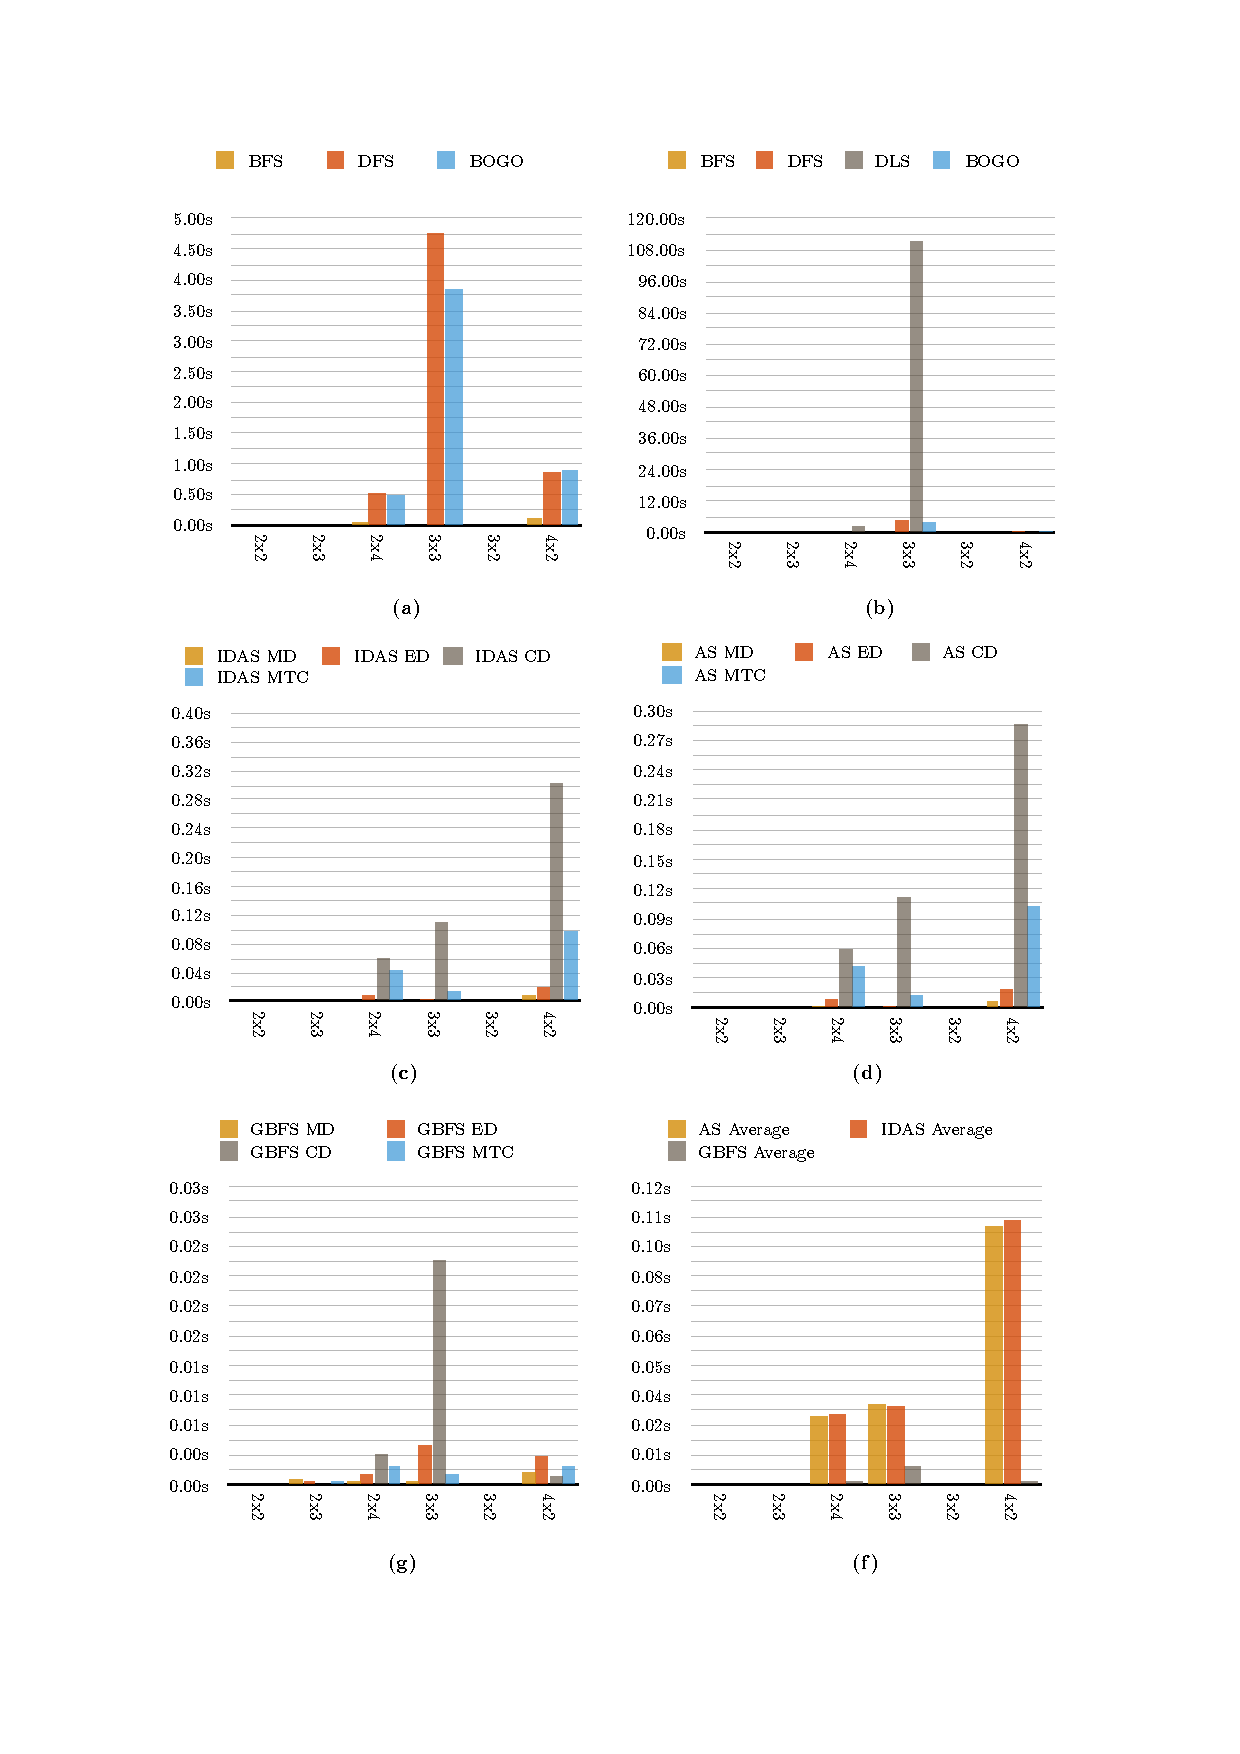
\includegraphics[width=0.8\textwidth]{graph.pdf}
  \caption{Aggregated results of performance tests}
  \label{fig:results}
\end{figure}

On analysis of Figure~\ref{fig:results}, it can be determined that the $3 \times 3$
states take the longest for most tests. This is understandable since the maximum
number of solvable states, $n$, for these tests are larger than all others:


\begin{center}
  \vspace{0.5em}
  \noindent
  $n_{3 \times 3} = \frac{( 3 \times 3 )!}{2} = 181440 > n_{2 \times 4} = \frac{( 2 \times 4 )!}{2} = 20160$
  \vspace{0.5em}
\end{center}

Figure~\ref{fig:results}(b) highlights that \texttt{DLS} is indeed the slowest
implemented algorithm, taking up to 110s to solve for a $3 \times 3$ puzzle. This
may be caused by the node expansion test as implemented in Listing~\ref{lst:nodeexpand},
but is probably unlikely since the test is not an expensive or time-consuming
operation (a node's \texttt{pathCost} is not a computed property and would therefore
be an inexpensive integer reference).

\lstinputlisting[
  label=lst:nodeexpand,
  caption=
    Implementation of node expansion test for \texttt{DLS},
  language=swift,
  linerange=25-27
]{../../src/DepthLimitedSearch.swift}

\lstinputlisting[
label=lst:nodeexpand2,
caption=
Implementation of node expansion test for \texttt{IDAS},
language=swift,
linerange=25-27
]{../../src/IterativeDeepeningAStarSearch.swift}

Factoring this outlier out (Figure~\ref{fig:results}(a)), the \texttt{BFS} performs
best on each of the tests, followed second by \texttt{BOGO} and lastly \texttt{DFS}.

Similarly, the informed search that is depth-limited (\texttt{IDAS}) is also slower
than its non-depth-limited counterpart \texttt{AS}. Whilst \texttt{IDAS} is still far
improved than \texttt{GBFS} as shown in the summary Figure~\ref{fig:results}(f), it still
involves a similar node expansion test that \texttt{DLS} has (refer to
Listing~\ref{lst:nodeexpand2}).

Figures~\ref{fig:results}(c) to Figures~\ref{fig:results}(g) also show that the Chebyshev
distance is consistently the slowest-calculating heursitic to use for informed
searches. Manhattan and Euclidean distances are shown to be faster; this may
be due to their simplier implementations.
